\chapter{Ad Hoc and Sensor Networks}
In this section our aim is to study efficient algorithms to setting up a multihop communication in an ad hoc or sensor network.
In these type of networks multiple nodes, geographically random distributed and with very limited resources, need to communicate each others. For this reason it's important to take in account the energy/latency performance of the network.

In general, in a sensor network is a good practice to save as much power as possible, so we assume that a node $A$ can be in \textit{active} or in \textit{sleep} mode.
\textit{Active mode} includes three state:
\begin{itemize}
	\item \textit{trasmitting state}: node $A$ is transmitting data to another node $B$ with a consequent power consumption;
	\item \textit{receiving state}: node $A$ is receiving data from another node $B$, here $A$ have to perform at least some decoding operations on the incoming packets;
	\item \textit{idle state}: node $A$ is listening to the channel to sense for new incoming request of communication, that is implemented with a busy waiting (and power consumption).
\end{itemize}

\textit{Sleep mode} is a way to avoid useless power consumption. When a node is in this state, it switch off most of its hardware, keeping active just some core feature like clock. It can't receive or listen for anything.
\begin{figure}[h]
\centering
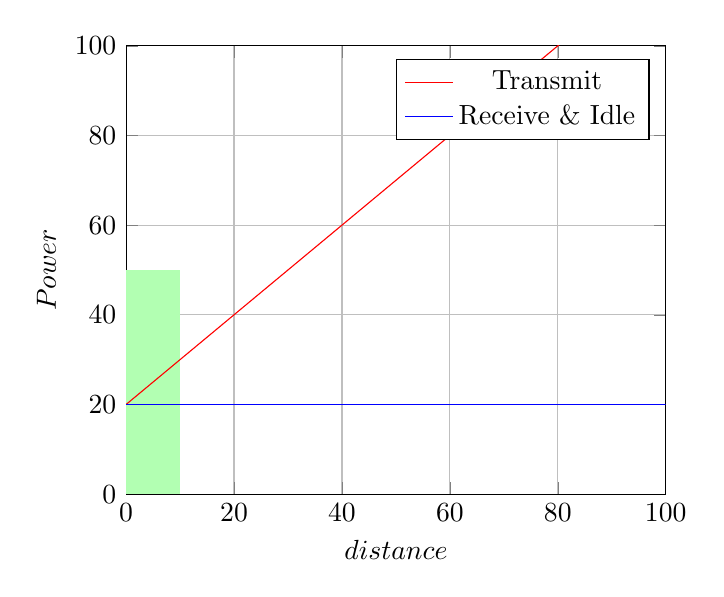
\begin{tikzpicture}
	\begin{axis}[
	xmin = 0, xmax = 100,
	ymin = 0, ymax = 100,
	grid = major,
	xlabel = $distance$, ylabel = $Power$,
	legend pos=north east
	]
	\fill[green!30]
		(axis cs:0,0) --
		(axis cs:0,50) --
		(axis cs:10,50) --
		(axis cs:10,0) --
		cycle;
	% \addplot [thick,color=blue,fill=blue, fill opacity=0.5]coordinates {
	% 	(0, 0)
	% 	(10, 0)
	% 	(0, 100)
	% 	(10, 100)};
	\addplot[domain=0:100,red] {x+20};
	\addplot[domain=0:100,blue] {20};
	\legend{Transmit, Receive \& Idle}
	\end{axis}
\end{tikzpicture}
\caption{M1} \label{fig:powervar}
\end{figure}

\Fig{fig:powervar} show as for long range communication (like satellite communication), a node in trasmitting state consume more power than a node in receiving or in idle state, since decoding and listening operations are independent from the distance between transmitter and receiver, while transmission power grows with that distance\footnote{the growing rate is super linear, but here is shown as linear for sake of simplicity}.
Our aim is to focus on short range communication, in which the amount of power consumed in each of the three state is almost the same (as \Fig{fig:powervar} shows in the green rectangle), for this reason the only way to save power is introducing the \textit{sleep mode}.

How can the network be efficiently used under these assumption?

\section{SPAN Method}
\begin{figure}[h]
	\centering
	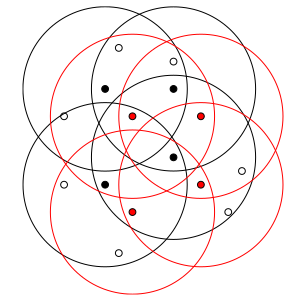
\includegraphics[width=0.4\textwidth]{SPAN.png}
	\caption{Sensor network subdivided into classes as required by SPAN method}
	\label{fig:SPAN}
\end{figure}

The set of nodes of a sensor network can be divided in $N$ subsets in a way to assign to each node a class.
Each class ensure a good communication across the network.
In this way each class of node can sleep $\frac{N-1}{N}$ of the time.
This behaviour is shown in \Fig{fig:SPAN}.

\begin{example}
	A network is divided in 3 classes of nodes $\Rightarrow$ each class can sleep $2/3$ of the time.
\end{example}

The drawback for this method is that each node must know which class it belongs to, so a global coordination is required. This is an unfeasible requirement in networks with thousands of nodes.

\section{GAF Method}
\begin{figure}[h]
	\centering
	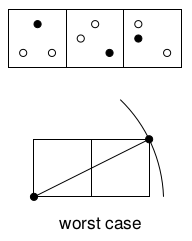
\includegraphics[width=0.4\textwidth]{GAF.png}
	\caption{GAF behaviour in a sensor networks}
	\label{fig:GAF}
\end{figure}
GAF is similar to SPAN in a sense since it envisions the use of only a fraction of the nodes at any given time. The
specific approach of GAF is to divide the area in square
regions, called grids, in such a way that any two nodes in
neighboring grids are within range of each other, and in each grid at least a node is awaken. With this approach each grid can work independently from the others, so a global coordination is not required. The GAF scheme is presented in \Fig{fig:GAF}.

The price to pay is that for every configuration we take two adiacent nodes (when two nodes in neighboring grids are at the maximum distance each other), the hop length is significantly smaller than the radio range. This may result in inefficiency in terms of latency and energy consumption (more hops than possibly needed).

\section{STEM Method}
\begin{figure}[h]
	\centering
	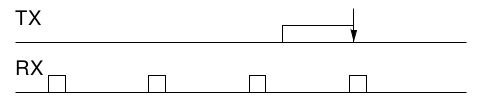
\includegraphics[width=0.6\textwidth]{STEM.png}
	\caption{STEM mechanism in a sensor networks}
	\label{fig:STEM}
\end{figure}
STEM method solves the problem of sleeping nodes by providing a rendezvous mechanism, using beacons and periodic wakeup.
Each sleeping node wakes up periodically to listen. If a node wants to establish communications, it starts sending out beacons polling a specific user. Within a bounded time, the polled node will wake up and receive the poll, after which the two nodes are able to communicate. This mechanism is shown in \Fig{fig:STEM}.

\section{Geographic Random Forwarding}
\begin{figure}[h]
	\centering
	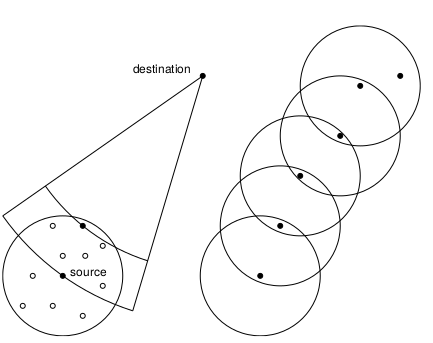
\includegraphics[width=0.6\textwidth]{GeRaF.png}
	\caption{Geographic Random Forwarding mechanism in a sensor networks}
	\label{fig:GeRaF}
\end{figure}
\gls{geraf} is based on knowledge of a node’s own position and of the position of the destination.
With this technique there's no need to explicitly address the next hop, since it choose the best hop between sensors awaken within the radio range of the source.

Given a node (source) that needs to communicate to another node (destination), the \textit{best hop} is the sensor within the radio range of the source, that is closest to the destination in terms of meters or kilometers.

This \textit{best hop} is chosen after the transmission has started, in the following method:
\begin{itemize}
	\item source send a broadcast message that contains the source and the destination position, all active nodes within its range receive it;
	\item each node determines its own priority as a relay, based on geometric considerations;
	\item contention phase takes place so that nodes closer to the destination are likely to win;
	\item the winner becomes itself the source.
\end{itemize}

This algorithm is iterated until the destination is reached, a scheme of this is shown in \Fig{fig:GeRaF}.

Since \gls{geraf} is based on geographically position of the nodes, it allow to reach the destination in less hop than GAF.

\subsection{Analytical approach}
	Given two areas A and B with different shape but the same area measure, the number of sensors in A depends on the measure of its area and not on its shape.

	Therefore the number of sensors in A and in B have the same distribution. We assume that this distribution is Poissonian, so for area A we can state:
	\begin{equation}
		\begin{split}
			number ~of ~sensors ~in ~A &= \lambda A \\
			\prob[0 ~nodes ~in ~A] = e^{-\lambda A}
		\end{split}
	\end{equation}

	\begin{figure}[h]
		\centering
		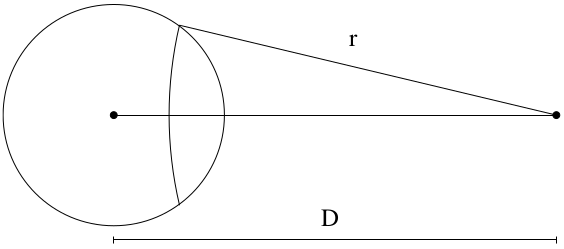
\includegraphics[width=0.8\textwidth]{analytical_scheme.png}
		\caption{Scheme of a sensors network}
		\label{fig:anapproach}
	\end{figure}

	% \begin{figure}[h]
	% 	\begin{tikzpicture}
	% 		\node (v2) at (-4,0) {\textbullet};
	% 		\node (v1) at (-13,0) {\textbullet};
	% 		\def\radius{2.5cm}
	% 		\draw  (v1) circle[radius=\radius];
	% 		\fill[red] (v1) +(160:\radius) {circle[radius=2pt]};
	% 		\node (v3) at (1.5,2) {\textbullet};
	% 		\draw  plot[smooth, tension=.7] coordinates {(v1) (v2)};
	% 	\end{tikzpicture}
	% 	\caption{title}
	% \end{figure}

	Given $\zeta$ the advancement between two nodes, with reference to \Fig{fig:anapproach}, $\zeta < D - r$ if there are no relays in circle intersection of area
	\begin{equation}
			A(r,D) = 2 \int_{D-1}^r a \cdot arccos\left( \frac{a^2 + D^2 - 1}{2aD}\right) da
	\end{equation}

	so we can define the statistic of the advancement $\zeta$ as
	\begin{equation}
		\prob[\zeta > a] = \begin{cases}
			0 & a \ge 1\\
			1-e^{-MA(D-a,D)/\pi} & otherwise
		\end{cases}
	\end{equation}

	where $M$ stands for $\lambda$. Given these quantities, we can define the average advancement towards the destination as

	\begin{equation}
		\exp[\zeta] = \int_0^{+\infty} \prob[\zeta > a]da = 1-\int_0^1 e^{\frac{-MA(D-a,D)}{\pi}}da
	\end{equation}

	and an approximation for the average number of hops as

	\begin{equation}
		\exp(n) \approx \frac{D}{\exp[\zeta]}
	\end{equation}

A rigorous way to compute $\exp[n]$ is the following.

\begin{equation}\label{hopsdefinition}
	\begin{split}
		&n' = \text{number of hops to reach node within coverage of the destination}\\
		&n = n' + 1 = \text{number of hops}
	\end{split}
\end{equation}

We can state

\begin{equation}\label{firstBound}
	\sum_{i=1}^{n'-1} X_i < D-1 \le \sum_{i=1}^{n'} X_i
\end{equation}

where $X_i$ are r.v. representing the advancement in a given hop.
This may seem like a \textit{stopping rule}, since I can advance until I enter in the range of the destination and $n'$ can be used as the \textit{stopping time}, but $X_i$ are neither independent nor identically distributed, since these depends on the distance from the source.

For the moment, we can ignore this problem and replace $X_i$ with an iid sequence $Y_i$, and replace it in \eq{firstBound}.

\begin{equation}\label{stoppingRule}
	\sum_{i=1}^{n'-1} Y_i < D-1 \le \sum_{i=1}^{n'} Y_i
\end{equation}

where $Y_i$ are iid.
In this way we can apply to \eq{stoppingRule} the stopping theory and divide the problem in two parts.

\begin{enumerate}
		\item
			$$ D-1 \le \exp\left[\sum_{i=1}^{n'} Y_i\right] \stackrel{(1)}{=} \exp[n']\exp[Y] $$
			Where (1) holds for the Wald's equation. Rearranging the previous equation and using \eq{hopsdefinition}, we can find that
			\begin{equation}\label{lowerBound}
				\exp[n] = \exp[n'+1] \ge \frac{D-1}{\exp[Y]} +1
			\end{equation}
		\item
			Advancement $\zeta$ is at most 1, then
			$$\sum_{i=1}^{n'} Y_i \le \sum_{i=1}^{n'-1} Y_i +1 \stackrel{(1)}{<} D$$
			Where (1) is derived from \eq{stoppingRule}. Then we can apply the expectation and the Wald's equation, obtaining
			$$\exp\left[\sum_{i=1}^{n'} Y_i\right] = \exp[n']\exp[Y] < D$$
			Then, applying the definition of number of hops in \eq{hopsdefinition} we obtain the second bound.
			\begin{equation}\label{upperBound}
				\exp[n] < \frac{D}{\exp[Y]} + 1
			\end{equation}

			The final result is the union of the bounds \eq{lowerBound} and \eq{upperBound}:
			\begin{equation}\label{iidBounds}
				\frac{D-1}{\exp[Y]} +1 \le \exp[n] < \frac{D}{\exp[Y]} + 1
			\end{equation}
\end{enumerate}
Then we must replace $Y$ with $X$ appropriately in the result.
If we assume that all the $X_s$ have the statistic of $X_1$(worst case), we have the maximum number of hops, while if we assume that all the $X_s$ have the statistic of $X_D$(best case) we have the minimum number of hops. So we can replace in \eq{iidBounds} the best and the worst case, obtaining the final result:

\begin{equation}\label{finalBounds}
	\underbrace{\frac{D-1}{\exp[X_d]} +1}_\text{Best Case} \le \exp[n] < \underbrace{\frac{D}{\exp[X_1]} + 1}_\text{Worst Case}
\end{equation}
